\documentclass[11pt,a4paper,fleqn]{scrartcl}

\usepackage[utf8]{inputenc}
\usepackage[T1]{fontenc}
\usepackage[colorlinks=true, citecolor=blue, linkcolor=blue, filecolor=blue,urlcolor=blue]{hyperref}
\hypersetup{
     colorlinks   = true,
     citecolor    = gray
}
\usepackage{wrapfig}

\usepackage{caption}
\captionsetup{format=plain, indent=5pt, font=footnotesize, labelfont=bf}

\setkomafont{disposition}{\scshape\bfseries}

\usepackage{amsmath}
\usepackage{amssymb}
\usepackage{amsfonts}
%\usepackage{bbm}
% \usepackage{mathtools}
% \usepackage{epsfig}
% \usepackage{grffile}
%\usepackage{times}
%\usepackage{babel}
\usepackage{tikz}
\usepackage{paralist}
\usepackage{color}
\usepackage[top=3cm, bottom=2.5cm, left=2.5cm, right=3cm]{geometry}
%\setlength{\mathindent}{1ex}

% PGF
\usepackage{pgfplots}
\usepackage{pgf}
\usepackage{siunitx}
\usepackage{xfrac}
\usepackage{calculator}
\usepackage{calculus}
\usepackage{eurosym}
\usepackage{booktabs}
%\sisetup{per-mode=fraction,%
%	fraction-function=\sfrac}

%\newcommand{\eur}[1]{\EUR{#1}\si{\per\kilo\meter}}
\pgfplotsset{
  compat=newest,
  every axis/.append style={small, minor tick num=3}
}

%\usepackage[backend=biber,style=alphabetic,url=false,doi=false]{biblatex}
%\addbibresource{sheet01_biber.bib}
% \addbibresource{/home/coroa/papers/refs.bib}

\newcommand{\id}{\mathbbm{1}}
\newcommand{\NN}{{\mathbbm{N}}}
\newcommand{\ZZ}{{\mathbbm{Z}}}
\newcommand{\RR}{{\mathbbm{R}}}
\newcommand{\CC}{{\mathbbm{C}}}
\renewcommand{\vec}[1]{{\boldsymbol{#1}}}

\renewcommand{\i}{\mathrm{i}}

\newcommand{\expect}[1]{\langle\,#1\,\rangle}
\newcommand{\e}[1]{\ensuremath{\,\mathrm{#1}}}

\renewcommand{\O}{\mc{O}}
\newcommand{\veps}{\varepsilon}
\newcommand{\ud}[1]{\textup{d}#1\,}

\newcommand{\unclear}[1]{\color{green}#1}
\newcommand{\problem}[1]{\color{red}#1}
\newcommand{\rd}[1]{\num[round-mode=places,round-precision=1]{#1}}

%\DeclareSIUnit{\euro}{\EUR}
\DeclareSIUnit{\dollar}{\$}
\newcommand{\eur}{\text{\EUR{}}}

\usepackage{palatino}
\usepackage{mathpazo}
\setlength\parindent{0pt}
\usepackage{xcolor}
\usepackage{framed}
\definecolor{shadecolor}{rgb}{.9,.9,.9}

\def\cap{\text{Cap}}
\def\floor{\text{Floor}}
\def\l{\lambda}
\def\m{\mu}
\def\d{\partial}
\def\cL{\mathcal{L}}
\def\co2{CO${}_2$}

\def\mw{\text{ MW}}
\def\mwh{\text{ MWh}}
\def\gw{\text{ GW}}
\def\gwh{\text{ GWh}}
\def\emwh{\text{ \euro/MWh}}
\def\bemwh{\text{ [\euro/MWh]}}
\newcommand{\ubar}[1]{\text{\b{$#1$}}}

%=====================================================================
%=====================================================================
\begin{document}

\begin{flushright}
  \textbf{Energy Systems}\\
  {\small Technical University of Berlin}\\
  {\small Department of Digital Transformation in Energy Systems}\\
  {\small Summer Term 2021}\\
 \end{flushright}
 
  
  \vspace{-0.5em}
  \hrulefill
  \vspace{0.3em}
 
 \begin{center}
  \textbf{\textsc{\Large Solutions IV: Electricity Markets}}\\
  \small Will be worked on in the exercise session on Friday, 25 June 2020.\\[1.5em]
 \end{center}
 

 \vspace{-0.5em}
 \hrulefill
 \vspace{0.8em}
 

%=============== ======================================================
\paragraph{Solution IV.1 \normalsize (Shadow prices of limits on consumption).}~\\
%=====================================================================

Suppose that the utility for the electricity consumption of an industrial company is given by
\[
U(d) = 70d - 3d^2 [\textrm{\euro}/\si{\hour}] \quad , \quad d_{min}=2\leq d \leq d_{max}=10,
\]
where $d$ is the demand in MW and $d_{min}, d_{max}$ are the minimum and maximum demand. \\
[1em]
Assume that the company is maximising its net surplus for a given electricity price $\pi$, i.e. it maximises $\max_{d} \left[U(d) -
\pi d\right]$.
\begin{enumerate}[(a)]
 \begin{shaded} \item If the price is $\pi = 5$~\euro/MWh, what is the optimal
  demand $d^*$?  What is the value of the KKT multiplier $\mu_{max}$
  for the constraint $d \leq d_{max}=10$ at this optimal solution?
  What is the value of $\mu_{min}$ for $d \geq d_{min} = 2$?\end{shaded}
%%%%%%%%%%%%%%%%%%%%%%%%%%%%%%%%%%%%%%%%%%%%%%%%%%%%%%%%%%%%
%%%%%%%%%%%%%%%%%%%%%%%%%%%%%%%%%%%%%%%%%%%%%%%%%%%%%%%%%%%%%%%%%%%%%%%%%%%%%%%%%
 We convert the exercise to an optimisation problem with objective
 \begin{align}
  &f(d) = U(d) - \pi d = (70-\pi) d - 3d^2 \\
  &\max\limits_{d \in \mathbb{R}} \ f(d)
 \end{align}

 with constraints
 \begin{align}
  d  & \leq d_{max} = 10 \hspace{1cm}\leftrightarrow\hspace{1cm} \m_{max}  \\
  -d & \leq -d_{min} = -2 \hspace{1cm}\leftrightarrow\hspace{1cm} \m_{min}
 \end{align}
 \rule{\textwidth}{0.4pt}
%%%%%%%%%%%%%%%%%%%%%%%%%%%%%%%%%%%%%%%%%%%%%%%%%%%%%%%%%%%%%%%%%%%%%%%%%%%%%%%%%
 From stationarity for the optimal point we get:
 \begin{align}
  0 & =   \frac{\d \mathcal{L}}{\d d} = \frac{\d f}{\d d} - \sum_{i} \lambda_i^* \frac{\d g_i}{\d d} -  \sum_{j} \mu_j^* \frac{\d h_j}{\d d}\\
  0 & =   \frac{\d}{\d d} \left((70-\pi) d - 3d^2 \right) - \m_{max} + \m_{min} \\
    & =  (70-\pi) - 6d - \m_{max} + \m_{min} \label{eq:2stat}
 \end{align}

 Note that it does not matter whether you pull in the constant of the right-hand side of the respective constraint.
%%%%%%%%%%%%%%%%%%%%%%%%%%%%%%%%%%%%%%%%%%%%%%%%%%%%%%%%%%%%%%%%%%%%%%%%%%%%%%%%%%%%%%%%
\begin{figure}[h]
	\centering
	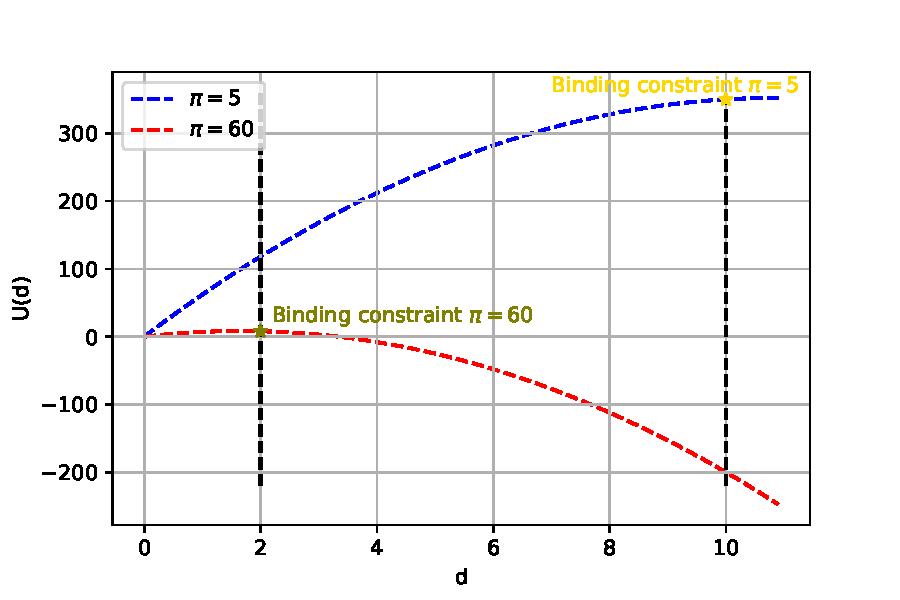
\includegraphics{graph_u_problem1.pdf}
	\caption{utility for the electricity consumption with demand d}
	\label{fig:solution04tutorial}
\end{figure}
%%%%%%%%%%%%%%%%%%%%%%%%%%%%%%%%%%%%%%%%%%%%%%%%%%%%%%%%%%%%%%%%%%%%%%%%%%%%%%%%%%
 The marginal utility curve is $U'(d) = 70 - 6d$ [\euro/MWh]. At
 $\pi = 5$ and if the demand were unconstrained, the demand would be determined by $5=70-6d$, i.e. $d =
  65/6 = 10.8333$, which is above the consumption limit
 $d_{max} = 10$. Therefore the optimal demand is \\
  $d^* = 10$,\\
   the upper limit is binding such that $\mu_{max} \geq 0$ and the lower limit is non-binding such that\\
    $\mu_{min} = 0$. \\
%%%%%%%%%%%%%%%%%%%%%%%%%%%%%%%%%%%%%%%%%%%%%%%%%%%%%%%%%%%%%%%%%%%%%%%%%%
 To determine the value of $\mu_{max}$ we use \eqref{eq:2stat} to get
 \begin{equation*}
	\m_{max} =  (70-\pi) - 6d^* - \mu_{min} =  70 - 5 -60 = 5
 \end{equation*}
%%%%%%%%%%%%%%%%%%%%%%%%%%%%%%%%%%%%%%%%%%%%%%%%%%%%%%%%%%%%%%%%%%%%%%%%%%%

 \begin{shaded}
  \item Suppose now the electricity price is $\pi = 60$~\euro/MWh. What are
  the optimal demand $d^*$, $\mu_{max}$ and $\mu_{min}$ now?
 \end{shaded}
%%%%%%%%%%%%%%%%%%%%%%%%%%%%%%%%%%%%%%%%%%%%%%%%%%%%%%%%%%%%%%%%%%%%%%%%%%
 At $\pi = 60$, the demand would be determined by $60=70-6d$, i.e. $d = 10/6 = 1.667$, which is below the consumption limit $d_{min} = 2$. Therefore the optimal demand is \\
  $d^* = 2$,\\
   the upper limit is non-binding such that\\
    $\mu_{max}= 0$\\
 and the lower limit is binding such that $\mu_{min} \geq 0$.

 To determine the value of $\mu_{min}$ we use \eqref{eq:2stat} to get
 \begin{equation*}
   \m_{min} = -(70-\pi) + 6d^* + \mu_{max} = -(70 - 60) + 12 + 0 = 2.
 \end{equation*}
 
 \newpage
\end{enumerate}
%%%%%%%%%%%%%%%%%%%%%%%%%%%%%%%%%%%%%%%%%%%%%%%%%%%%%%%%%%%%%%%%%%%%%%%%%%%%%%%
%=============== ======================================================
\paragraph{Solution IV.2 \normalsize (Economic dispatch in a single bidding zone).}~\\
%=====================================================================

Consider an electricity market with two generator types, one with the cost function $C_1(g_1)=c_1g_1$ with variable cost $c_1 = 20\emwh$, capacity $G_1 = 300\mw$ and a dispatch rate of $g_1$~[MW], and another with the cost function $C_2(g_2)=c_2g_2$ with variable cost $c_2=50\emwh$, capacity $G_2=400\mw$ and a dispatch rate of $g_2$~[MW]. The demand has utility function $U(d) = 8000d - 5d^2$~[\euro/h] for a consumption rate of $d$~[MW].
\begin{enumerate}[(a)]
 \begin{shaded}\item What are the objective function and constraints required for an optimisation problem to maximise short-run social welfare in this market?\end{shaded}

 The optimisation problem has the objective function:
 \begin{align*}
 &f(d, g_1, g_2) =  U(d) - C_1(g_1) - C_2(g_2) = 8000d-5d^2 - c_1g_1 - c_2g_2 \\
 & \max_{d,g_1,g_2}f(d, g_1, g_2)
 \end{align*}
 with constraints:
 \begin{align*}
  d - g_1 - g_2 & = 0 \leftrightarrow \l              \\
  g_1           & \leq G_1 \leftrightarrow \bar{\m}_1 \\
  g_2           & \leq G_2 \leftrightarrow \bar{\m}_2 \\
  -g_1          & \leq 0 \leftrightarrow \ubar{\m}_1  \\
  -g_2          & \leq 0 \leftrightarrow \ubar{\m}_2
 \end{align*}
%%%%%%%%%%%%%%%%%%%%%%%%%%%%%%%%%%%%%%%%%%
 \begin{shaded}\item Write down the Karush-Kuhn-Tucker (KKT) conditions for this problem.\end{shaded}

\textbf{ Stationarity} gives for $d$:
 \begin{align*}
   0 & =   \frac{\d \mathcal{L}}{\d d} = \frac{\d f}{\d d} - \sum_{i} \lambda_i^* \frac{\d g_i}{\d d} -  \sum_{j} \mu_j^* \frac{\d h_j}{\d d}\\
   &= \frac{\d U}{\d d} - \l \\
   & = 8000 - 10d - \l 
 \end{align*}
 Stationarity for $g_1$ gives:
 \begin{equation*}
  -\frac{\d C_1}{\d g_1} + \l - \bar{\m}_1 + \ubar{\m_1}  =  -c_1+ \l - \bar{\m}_1 + \ubar{\m_1} = 0
 \end{equation*}
 Stationarity for $g_2$ gives:
 \begin{equation*}
  -\frac{\d C_2}{\d g_2} + \l - \bar{\m}_2 + \ubar{\m_2}  =  -c_2+ \l - \bar{\m}_2 + \ubar{\m_2} = 0
 \end{equation*}
\textbf{ Primal feasibility} is just the generator limits above in (a). \\
 \textbf{Dual feasibility} is $\bar{\m}_i^*,\ubar{\m}_i^* \geq 0$ and \\
  \textbf{complementary slackness} is $\bar{\m}_i^*(g_i^*-G_i) = 0$ and $\ubar{\m}_i^* g_i^* = 0$ for $i=1,2$.
%%%%%%%%%%%%%%%%%%%%%%%%%%%%%%%%%%%%%%%%%%%%%%%%%%%%%%%%%%%%%%%
 \begin{shaded}\item Determine the optimal rate of production of the generators and the value of all KKT multipliers. What is the interpretation of the respective KKT multipliers?\end{shaded}
 The marginal utility at the full output of the generators,
 \begin{align*}
 &G_1 + G_2 = 300\ \text{MW} + 400\ \text{MW} = 700\ \text{MW} \\
 &U'(700) = 8000 - 10\cdot700 = 1000\ \text{\euro/MWh}
 \end{align*}  
 which is higher than the costs $c_i$, so we'll find optimal rates
 \begin{align*}
 g_1^* &= G_1 = 300 \ \text{MW} \\
 g_2^* &= G_2 = 400 \ \text{MW} \\
 d^* &= G_1+G_2 = 700\ \text{MW} 
 \end{align*}
This means (from stationarity)
\begin{equation*}
\l^*= \frac{\d U}{\d d} \bigg|_{d=d^*} = 8000 - 10d^* = 1000 \text{\euro/MWh},
\end{equation*} 
which is the market price. Because the lower constraints on the generator output are not binding, from complementary slackness we have $\ubar{\m}_i = 0$. The upper constraints are binding, so $\bar{\m}_i \geq 0$. \\
 From stationarity $\bar{\m}_i =
  \l - c_i + \ubar{\m}_i$, which is the increase in social welfare if Generator $i$
 could increase its capacity by a marginal amount.

 $$\bar{\m}_1=1000-20=980 \text{\euro/MWh}$$
 $$\bar{\m}_2=1000-50=950 \text{\euro/MWh}$$

\end{enumerate}
\newpage
%=============== ======================================================
\paragraph{Solution IV.3 \normalsize (efficient dispatch in a two-bus power system).}~\\
%=====================================================================

\begin{figure}[h]
 \centering
 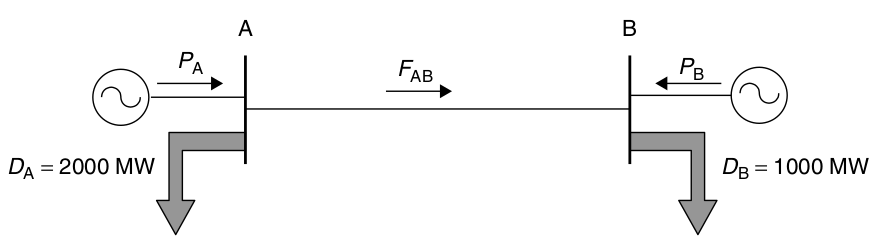
\includegraphics[width=14cm]{two-bus}
 \caption{A simple two-bus power system.}
 \label{twobus}
\end{figure}

Consider the two-bus power system shown in Figure \ref{twobus}, where the two nodes represent two markets, each with different total demand $D_i$, and one generator at each node producing $G_i$. At node A the demand is $D_A = 2000 \si{\mega\watt}$, whereas at node B the demand is $D_B = 1000 \si{\mega\watt}$. Furthermore, there is a transmission line with a capacity denoted by $F_{AB}$. The marginal cost of production of the generators connected to buses A and B are given respectively by the following expressions:
\begin{align*}
 MC_A & = 20 + 0.03 P_A \hspace{1cm}\eur/\si{\mega\watt\hour}  \\
 MC_B & = 15 + 0.02 P_B \hspace{1cm} \eur/\si{\mega\watt\hour}
\end{align*}

Assume that the demands $D_A$ and $D_B$ are constant and insensitive to price, that energy is sold at its marginal cost of production and that there are no limits on the output of the generators.

\begin{enumerate}[(a)]
 \begin{shaded}\item Calculate the price of electricity at each bus, the production
  of each generator, and the flow on the line for the following cases. You may also calculate the values of any KKT multiplier as a bonus.\end{shaded}

The price of electricity is the value of the dual variable at the nodal balance equation.

 Use the following nomenclature: price $\lambda_{A/B}$, generation $G_{A/B}$, flow $F_{AB}$.
 \begin{enumerate}[(i)]
  \begin{shaded}\item The line between buses A and B is disconnected.\end{shaded}

  Where to start: $P_A=D_A$ and $P_B=D_B$ and substitute into $MC_i$.

  $\l_A= 80\emwh$, $\l_B=35\emwh$,

  $G_{A}=2000$ MW, $P_B=1000$ MW, $F_{AB}=0$

  \begin{shaded}\item The line between buses A and B is in service and has an unlimited capacity.\end{shaded}
  
  Where to start:
  No restriction in transmission, so prices must be the same for the two nodes: $\l_A = \l_B$, therefore, $MC_A = MC_B$.
  Also: $P_A+P_B = D_A+D_B$.

    $\l_A= 53\emwh$, $\l_B=53\emwh$,

  $G_{A}=1100\mw$, $P_B=1900$ MW, $F_{AB}=-900\mw$

  \begin{shaded}\item The line between buses A and B is in service and has an unlimited capacity, but the maximum output of Generator B is 1500~MW.\end{shaded}
  
  Where to start:
  $P_B=1500$ MW since it is now constrained but would have been higher in the unconstrained case (ii). 
  Also, since there are no transmission constraints: $\l_A = \l_B$.
  Also: $P_A+P_B = D_A+D_B$.

    $\l_A= 65\emwh$, $\l_B=65\emwh$,

  $G_{A}=1500\mw$, $P_B=1500$ MW, $F_{AB}=-500\mw$

  \begin{shaded}\item The   line between buses A and B is in service and has an unlimited capacity, but the maximum output of Generator A is 900~MW. The output of Generator B is unlimited.\end{shaded}
  
  Where to start: 
  $P_A=900$ MW since it is now constrained but would have been higher in the unconstrained case (ii). 
  Also, since there are no transmission constraints: $\l_A = \l_B$.
  Also: $P_A+P_B = D_A+D_B$.

    $\l_A= 57\emwh$, $\l_B=57\emwh$,

  $G_{A}=900\mw$, $P_B=2100$ MW, $F_{AB}=-1100\mw$

  \begin{shaded}\item The line between buses A and B is in service but its capacity is limited to 600~MW. The output of the generators is unlimited.\end{shaded}
  
    Where to start:
    $F_{AB} = - 600$ MW since we would want even more transmission, if it were not constrained.
    Also, $P_A+F_{AB}=2000$ MW.

    $\l_A= 62\emwh$, $\l_B=47\emwh$,

  $G_{A}=1400\mw$, $P_B=1600$ MW, $F_{AB}=-600\mw$
 \end{enumerate}
 \begin{shaded}\item Calculate the generator revenues, generator profits, consumer payments and consumer net surplus for all the cases considered in the above problem. Who benefits from the line connecting these two buses?\end{shaded}
 Generator revenues $R_{i}$, generator costs $C_{i}$, generator profits $P_{i}$, consumer payments $E_{i}$. Find the generator profits by subtracting the costs from the revenue. Costs are given by integrating the marginal cost, i.e. $C_A = 20P_A + 0.015P_A^2$ and $C_B = 15P_B + 0.01P_B^2$. The generator at $B$ and the consumers at $A$ benefit from the line (price increases at $B$, decreases at $B$).
 \begin{table}[!h]
  \centering
  \begin{tabular}{lrrrrr}
   \toprule
   Case          & (i)      & (ii)     & (iii)    & (iv)     & (v)      \\
   \midrule
   $E_A$ (\euro) & 160,000 & 106,000 & 130,000 & 114,000 & 124,000 \\
   $R_A$ (\euro) & 160,000 & 58,300  & 97,500  & 51,300  & 86,800  \\
   $C_A$ (\euro) & 100,000 & 40,150  & 63,750  & 30,150  & 57,400  \\
   $P_A$ (\euro) & 60,000  & 18,150  & 33,750  & 21,150  & 29,400  \\
   \midrule
   $E_B$ (\euro) & 35,000  & 53,000  & 65,000  & 57,000  & 47,000  \\
   $R_B$ (\euro) & 35,000  & 100,700 & 97,500  & 119,700 & 75,200  \\
   $C_B$ (\euro) & 25,000  & 64,600  & 45,000  & 75,600  & 49,600  \\
   $P_B$ (\euro) & 10,000  & 36,100  & 52,500  & 44,100  & 25,600  \\
   \bottomrule
  \end{tabular}
 \end{table}

 \begin{shaded}\item Calculate the congestion surplus for case (v). For what values of the flow on the line between buses A and B is the congestion surplus equal to zero?\end{shaded}
 Congestion surplus is 9000 \euro:
 \begin{equation*}
  \left(E_A + E_B\right) - (R_A + R_B) = |F_{AB}|\times (\l_A - \l_B)
 \end{equation*}
 Congestion surplus is equal to zero when the flow $F_{AB}=0$, or when it is equal to the unconstrained value $F_{AB}=-900\mw$ (then $\l_A = \l_B$).
\end{enumerate}


\end{document}
